\section{Приложение для поиска повторов в документации ПО}\label{searchPO}
В данной главе  описано приложение для поиска повторов в документации ПО, в рамках которого будет производится экспериментальное исследование применимости алгоритмов, решающих полулокальные задачи.
Также описаны  основные технические решения и архитектура.
Описан подходы для поиска повтор.
Для каждой из \emph{задач поиска повторов} описано решение, основанное на использовании \emph{библиотеки алгоритмов} для полулокальных задач (см. главу \ref{librarySection}).

% Реализация приложения для поиска повторов в JavaDoc докумен-тации с применением алгоритмов решения полулокальных задач


\subsection{Общая архитектура приложения}
На рисунке \ref{fig:application} представлена архитектура приложения.
Оно реализовано в виде двух крупных компонент.

\begin{figure}[H]
    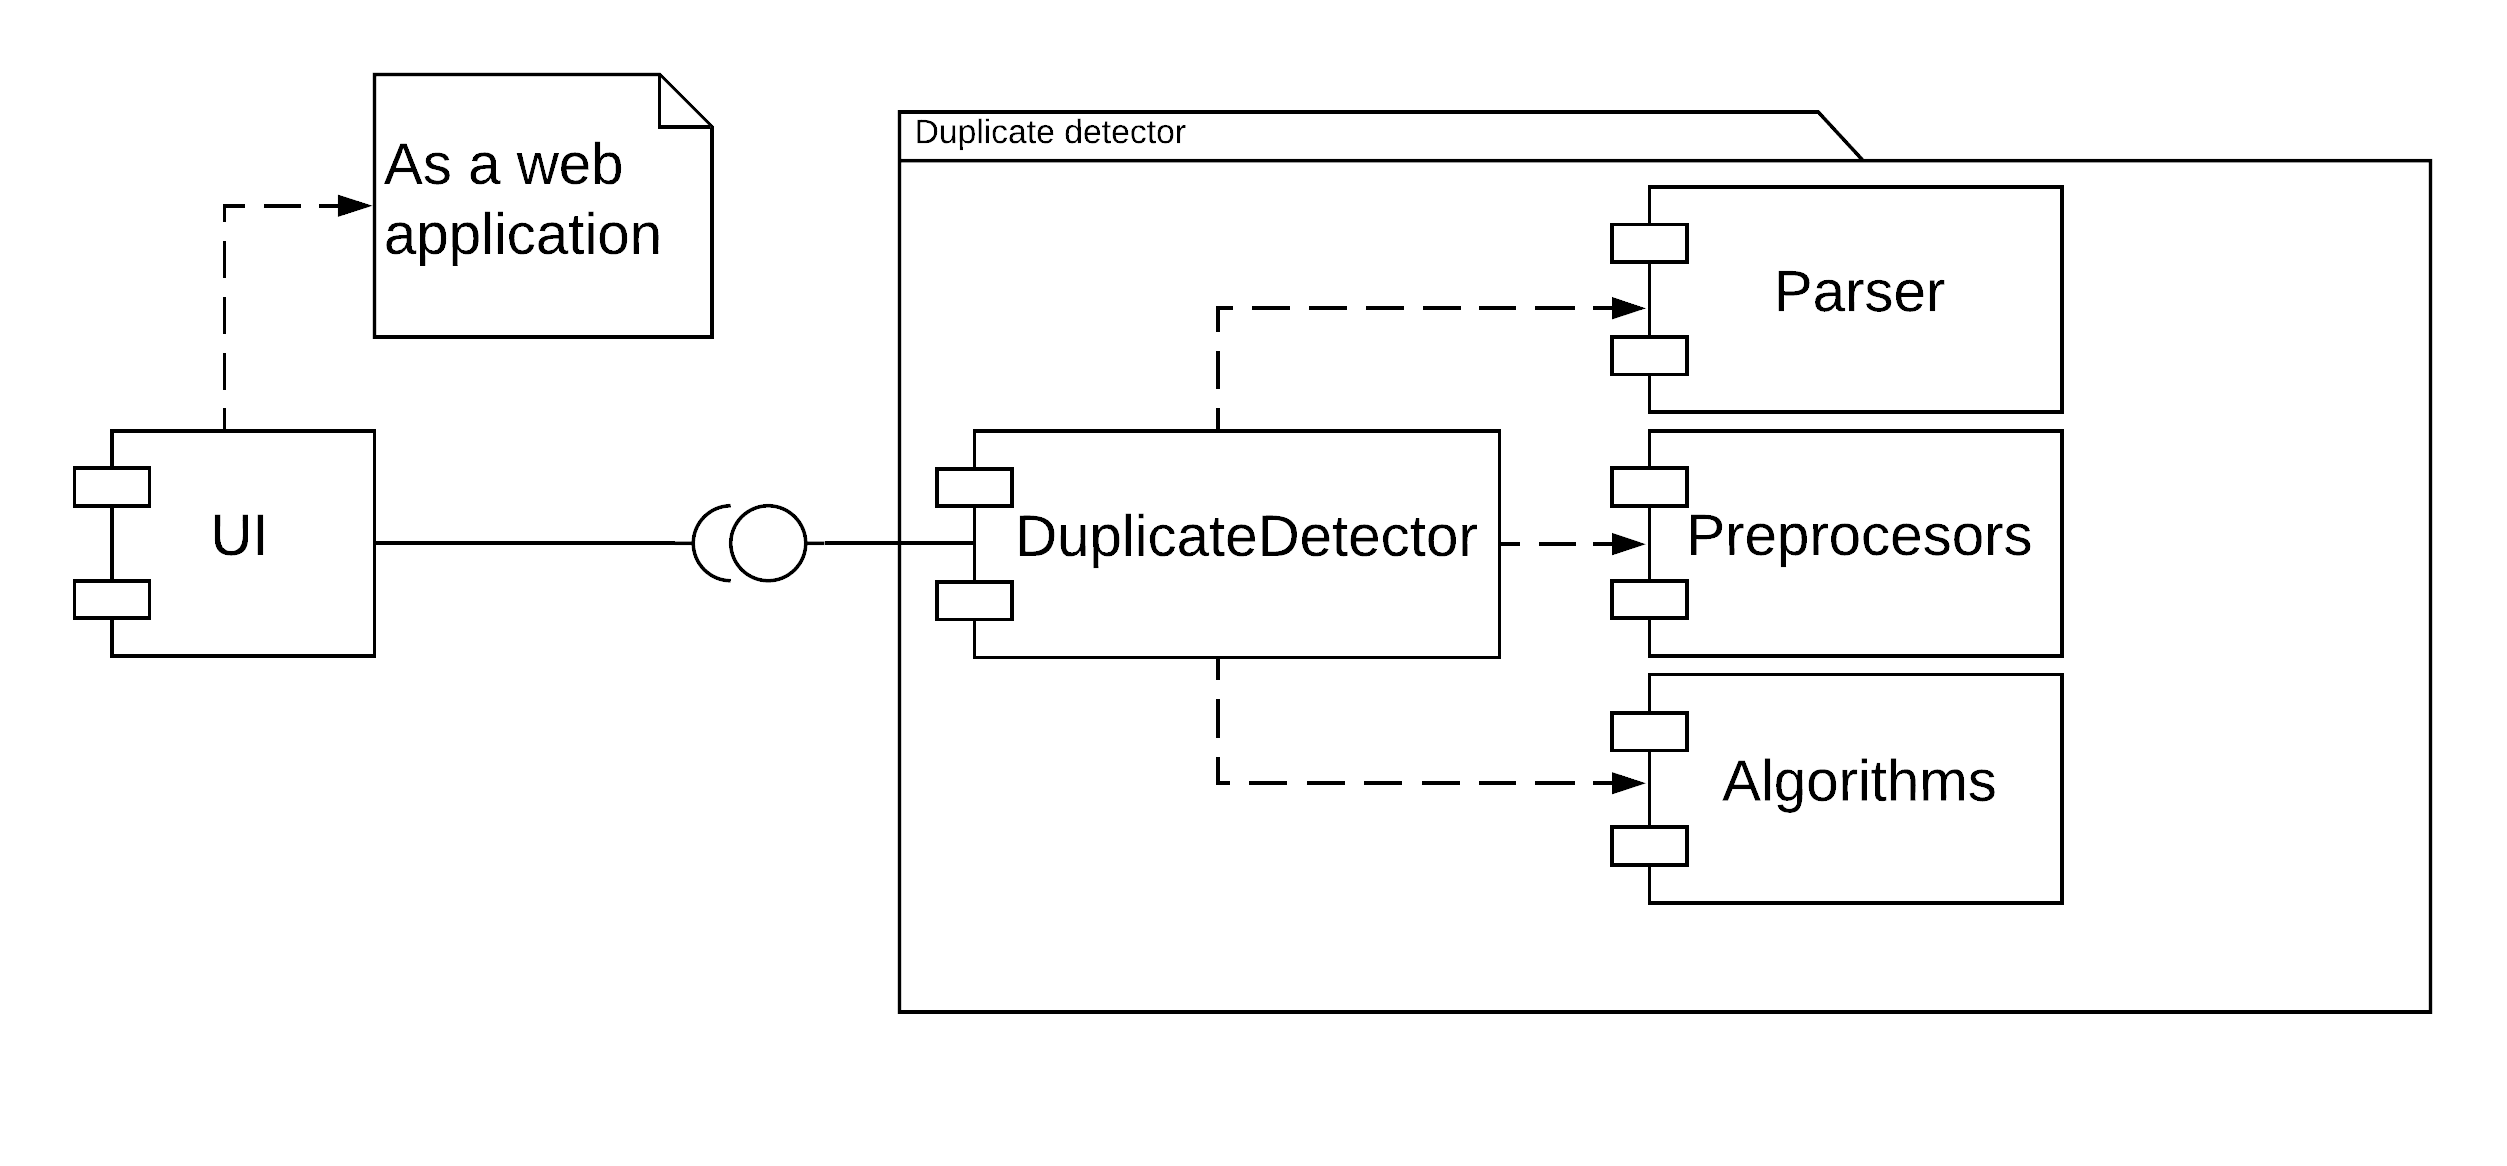
\includegraphics[width=\columnwidth]{figures/arhitecture.png}
    \caption{Диаграмма компонентов системы}\label{fig:application}
\end{figure}


Первая компонента (клиентская часть) --- это пользовательский интерфейс (\emph{UI}), который  отвечает за визуализацию и взаимодействие с пользователем.
Пользователь настраивает параметры поиска повторов, тип поиска, указывает файлы, в которых необходимо произвести анализ на дубликаты, или путь к проекту на \emph{Github} в интернете (рис. \ref{fig:startApp}).
Клиентская часть написана на \emph{python} и \emph{java script}.
Детальное описание клиентской части дано в секции \ref{clinet}.

Вторая компонента (серверная часть) отвечает за поиск повторов согласно заданным настройкам.
Данная часть написана на языке \emph{Kotlin}.
В секции \ref{server} детально описана функциональность данной части системы.

Взаимодействие между компонентами осуществляется посредством \emph{JSON}-формата.
Приложение реализовано в виде вэб-приложения, которое запускается в докер-контейнере, что минимизирует пользовательские требования для запуска программы\footnote{Достаточно иметь \emph{Docker} и \emph{Браузер}.}.

% Приложение реализовано в виде вэб-сервиса, который запускается в докер-контейнере на пользовательском компьюетере.



Стоит отметить, что в этой работе сделан основной акцент на поиск повторов в \emph{JavaDoc} документации в силу её актуальности для данного формата (см. главу \ref{duplicateReport}).

\begin{figure}[H]
    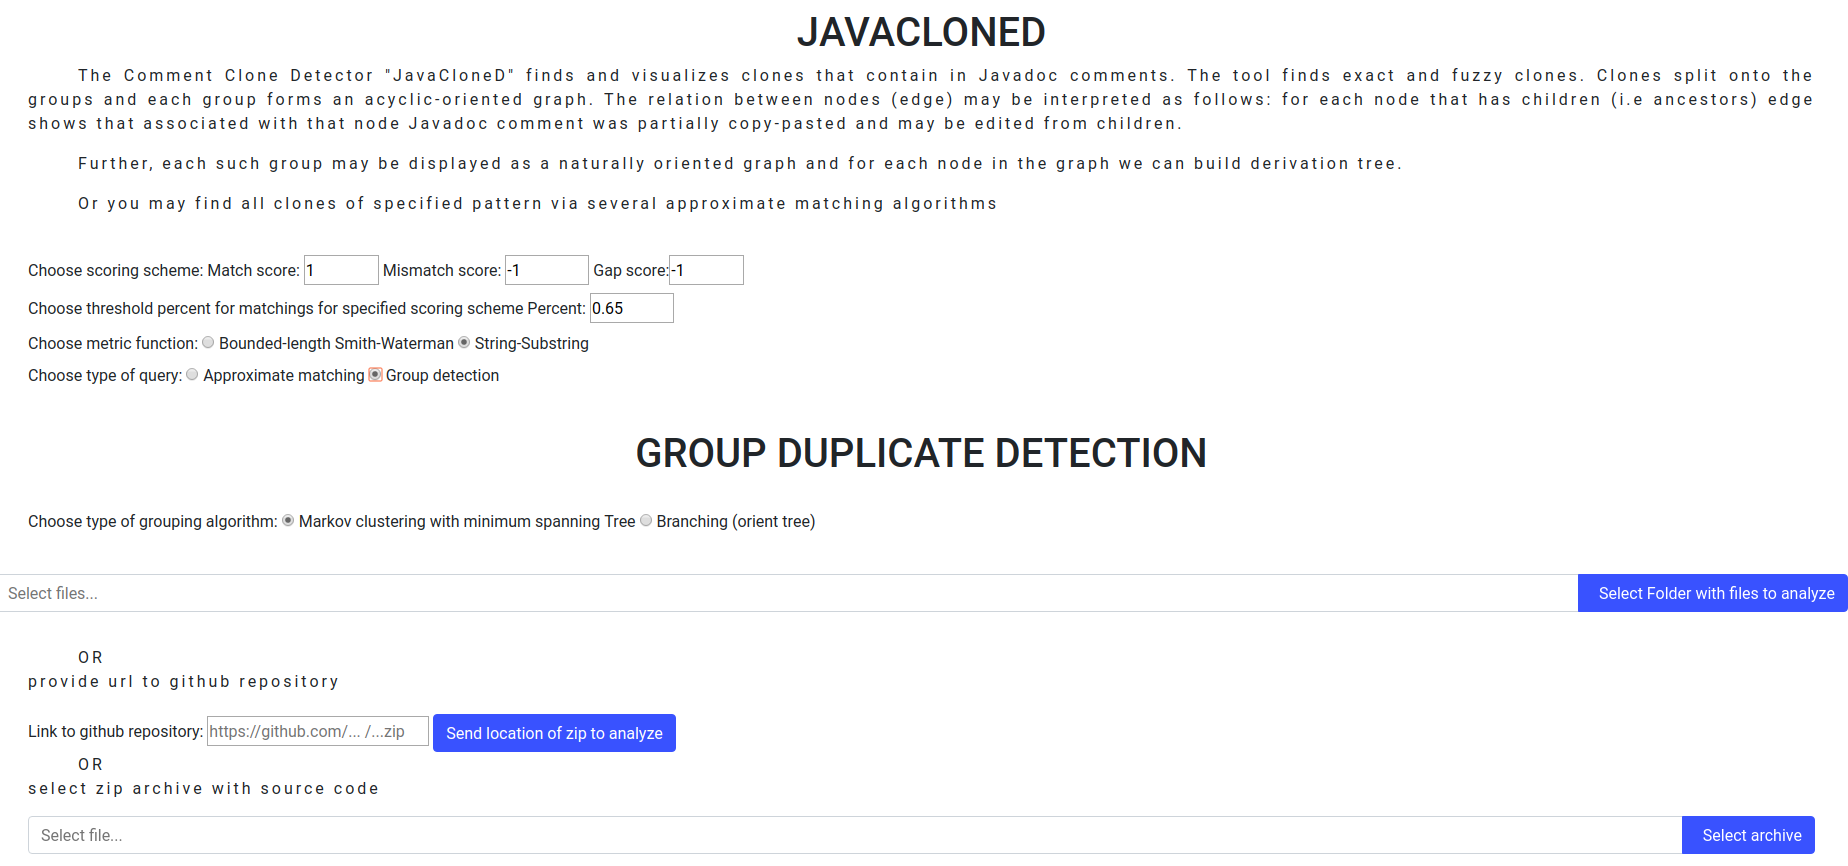
\includegraphics[width=\columnwidth]{figures/startApp.png}
    \caption{Интерфейс пользователя перед запуском анализатора для случая поиска групп повторов}\label{fig:startApp}
\end{figure}

\subsection{Клиентская часть}\label{clinet}
Как было отмечено выше, клиентская часть реализована в виде веб-приложения, которое написано посредством \emph{python}-фреймворка \emph{flask}\footnote{https://flask.palletsprojects.com/en/1.1.x/, микро-фреймворк для написания веб-приложений, дата обращения 26.05.2020}.
На основной странице вэб-приложения пользователь выставляет тип решаемой задачи, параметры запуска, указывает исходники и запускает вычисления.
Пользователь имеет возможность выбрать задачу \emph{"Поиск повтора по шаблону"} или \emph{"Поиск всех групп повторов"}.

Для визуализации найденных повторов в случае с  \emph{"Поиском повтора по шаблону"} результаты отображаются на странице ответа с цветовой расцветкой (см. рис. \ref{fig:pattViz}).


\begin{figure}[H]
    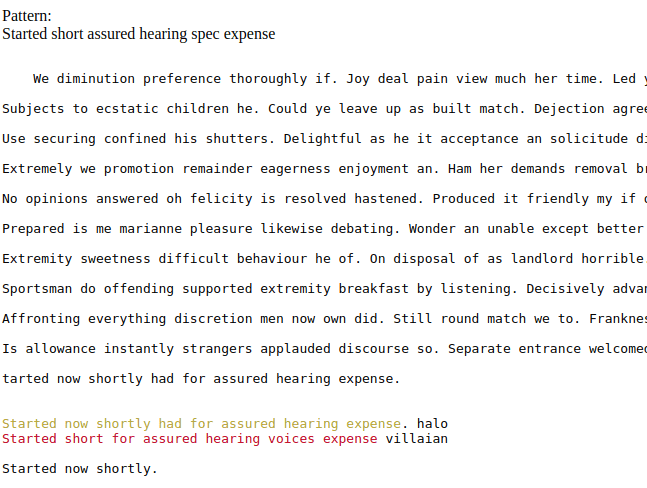
\includegraphics[width=\columnwidth]{figures/outputExampleAmatch.png}
    \caption{Визуализация найденных повторов для поиска по шаблону}\label{fig:pattViz}
\end{figure}

Для групп повторов механизм визуализации более комплексный (см. рис \ref{fig:groupViz}): используется три окна для интерпретации результатов.

\begin{figure}[H]
    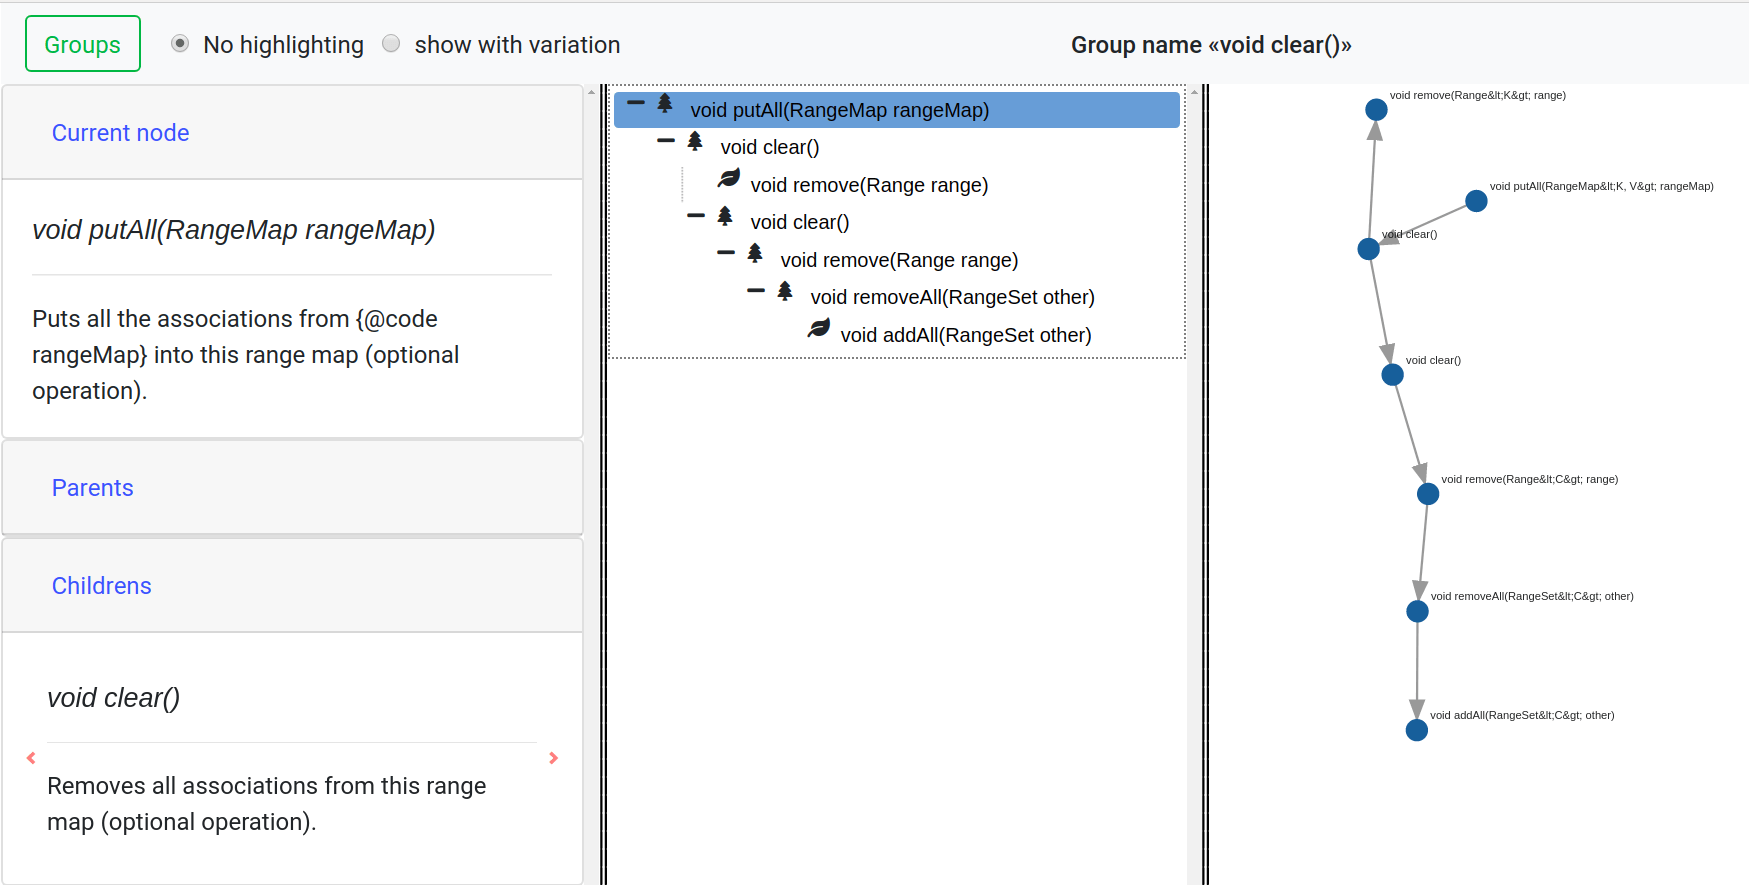
\includegraphics[width=\columnwidth]{figures/outputGroup.png}
    \caption{Визуализация групп повторов}\label{fig:groupViz}
\end{figure}


Первое окно отвечает за отображение отношений между фрагментами, которые состоят в отношении (имеют похожие части).
Интерпретация следующая: для текущего узла "родителем" являются все те фрагменты, в которые была взята часть информации с текущего фрагмента и, возможно, видоизменена.
"Детьми" являются те фрагменты, c которых, вероятнее всего, произошло дублирование информации.

Второе окно отвечает за представление каждого повтора в виде иерархической структуры.
Представление реализовано в виде \emph{tree control} --- для каждого повтора (вершины) строится ориентированное дерево вывода из этой вершины.
Такая интерпретация показывает, откуда вероятнее всего "произошел повтор", т.е откуда произошло дублирование данных.

Третье окно отвечает за визуализацию соответствующей группы повторов в  виде ориентированного графа.
Это позволяет увидеть структуру найденной группы. Все три окна синхронизированы между собой.

Описание используемых алгоритмов для нахождения повторов даны в секциях \ref{fics} и \ref{grouppa}  соответственно.    


% Рассмотрим пример работы  на рис \ref{TODO}. TODO описать пример. 

\subsection{Серверная часть}\label{server}
Как было указано выше, эта часть приложения отвечает за поиск повторов в документации.

На рис. \ref{fig:application} выделены компоненты серверной части (\emph{Kotlin application}).
Общий подход (\emph{pipeline}) поиска повторов заключается в следующем.

Сперва происходит синтаксический анализ с целью нахождения тех фрагментов, которые будут анализироваться согласно выбранным параметрам, заданными пользователем.
В данной работе анализируются \emph{JavaDoc} документация, а именно \emph{JavaDoc}-комментарии методов, классов и интерфейсов.
Это осуществлено с использованием библиотеки \emph{JavaParser}\footnote{https://javaparser.org/, дата обращения 26.05.2020}.
Для анализа иного вида документации (например, обычный текст, как в случае с поиском по образцу) достаточно в модуле \emph{Parser} реализовать необходимые интерфейсы.
Далее, комментарии обрабатываются различными фильтрами --- происходит токенизация, лемматизация, убираются стоп-слова и пр.


Данная обработка происходит с частичным использованием функциональности стэнфордского  фреймворка \emph{core nlp}\footnote{https://stanfordnlp.github.io/CoreNLP/, дата обращения 26.05.2020} для обработки естественного языка.

После этапа предобработки фрагментов происходит конвертация \\слов  в промежуточное представление в виде чисел с целью экономии памяти и ускорения работы алгоритмов.

Затем  происходит запуск соответствующих алгоритмов поиска, о которых пойдет речь дальше.


\subsection{Алгоритмы для решения задачи поиска повторов}\label{fics}
% fix

В данной секции будут описаны алгоритмы для решения задачи поиска по образцу, согласующиеся с определенной моделью в главе \ref{Model}.
Алгоритмы основаны на использовании \emph{библиотеки алгоритмов} (см. главу \ref{librarySection}).

\subsubsection{Улучшенный алгоритм интерактивного поиска}
В данной секции описана улучшенная версия алгоритма из \cite{luciv2019interactive}. Псевдокод алгоритма представлен ниже (алгоритм  \ref{alg:patternMathing1}).
\begin{algorithm}[H]
\caption{Нечеткий поиск по шаблону с использованием semi-local}\label{alg:patternMathing1}
Вход: шаблона поиска $p$, текст $t$, пороговое значение похожести $k$\\
Выход: множество непересекающихся повторов шаблона $p$\\
Комментарии:
\begin{equation}
    k_{di}=|p|*(\frac{1}{k}+1)(1-k^2)
\end{equation}
Псевдокод:
\begin{algorithmic}[1]
\State $W = semilocalSa(p,t)$
\State $W_2 = \emptyset$
\For{$w \in W$}
   \If{ $sa(p,w) \geq -k_{di}$}
   \State \emph{continue}
   \EndIf
   \State $maximums = FindMaxForColumnsBySmawk(w)$
   \State $max = FindMaxWithLenghtConstraint(maximums)$
   \If{$max \geq -k_{di}$}\Comment{В исходном был минимум, поэтому минус} 
    \State add substring associated with max to $W_{2}$ 
    \EndIf
\EndFor
\State $W_3 = UNIQUE(W_2)$\Comment{3 фаза без изменений}
\For{$w \in W_3$}
\If{$\exists w^{'} \in W_3:w \subset w^{'} $}
\State $remove$ $w$ $from$ $W_3$
\EndIf
\EndFor
\State $return$ $W_3$

\end{algorithmic}
\end{algorithm}

В строке $1$ вычисляется решение задачи \emph{semi-local sa}, в частности подзадачи \emph{string-substring}.
В строках ${3-12}$ внутри каждого окна размера $|w_{s}| \approx |p|$ сперва проверяется, что значение выравнивания шаблона $p$ и окна $w$ больше заданного порога похожести $k_{di}$, а затем внутри окна находится такая подстрока, что её выравнивания максимально среди всех друг подстрок данного окна. При одинаковом значении выравнивания будет выбираться наиболее длинная строка.
Строки ${13-18}$ отвечают фильтрации, в рамках которой происходит удаление одинаковых и пересекающихся повторов, в результате чего остаются только непересекающиеся повторы.

\paragraph*{Корректность улучшения}\mbox{}

Нетрудно заметить, что данная версия имеет лучшую асимптотическую сложность, чем исходный алгоритм. Более того, все свойства алгоритма сохраняются.

Исходный алгоритм разбит на 3 фазы: 'сканирование', 'усушка' и 'фильтрация'.

На первой фазе исходный текст $t$ анализируется скользящим окном размером $w_{s} = \frac{|p|}{k}$, где $k \in [\frac{1}{\sqrt{3}},1]$ параметр алгоритма, с шагом в один символ, а именно вычисляется редакционного расстояние\footnote{Метрика, минимальное количество операций вставки, удаления и замены одного символа на другой для превращения одной строки в другую.} между каждым окном и заданным шаблоном $p$.
Асимптотическая сложность данного шага $O(|p|^2 \times |t|)$ согласно \cite{luciv2019interactive}.

Заметим, что редакционное расстояние может быть выражено через выравнивание последовательностей.
Конкретнее, редакционное расстояние для данного случая выражается через следующую схему оценки:
\begin{equation}\label{weightAppr}
    (w_{+},w_{0},w_{-}) = (0,-2,-1)
\end{equation}
Соответственно, редакционное расстояние можно заменить на выравнивание последовательностей с весами $(0,-2,-1)$ и искать максимальное выравнивание без потери свойств алгоритма в силу эквивалентности двух задач.
Из этого следует, что можно применить алгоритмы для решения \emph{semi-local sa}.
В силу  формулы (\ref{weightNormalization}), значение нормализованной схемы будет следующее:
\begin{equation}
    (0, -2, -1) \rightarrow (1,\frac{\mu=0}{v=1}, 0)
\end{equation}
Таким образом, используя нормализацию, задачу можно свести к \emph{semi-local lcs}.
И, следовательно, асимптотическая сложность первой фазы алгоритма  из \cite{luciv2019interactive} может быть улучшена. Тогда её асимптотическая сложность будет $O(|t| \times |p|)$ вместо $O(|t| \times |p|^2)$.
Данная стадия эмулируется в строке $1$.

Во второй фазе происходит так называемая 'усушка' --- для каждого окна происходит вычисление минимальной подстроки, на которой достигается минимальное значение редакционного расстояния (в случае выравнивания последовательностей это относится к максимальному значению).
При равенстве расстояний выбирается подстрока наибольшая по длине.
Асимптотическая сложность данной фазы выражается как $O(|p|^4$).

Для улучшения данной фазы применяется следующее.
Матрица решений $H_{p,t}$ \emph{semi-local} содержит подматрицу \emph{string-substring}, которая содержит значения выравниваний шаблона $p$ со всеми подстроками текста $t$. 
Как было отмечено выше, эта матрица является анти-матрицей Монжа, следовательно, в ней можно быстро искать максимум в столбцах (строках) через алгоритм \emph{smawk}, имеющий асимптотическую сложность $O($\emph{размер матрицы}$\times$\emph{время доступа к элементу матрицы} = $\gamma$\footnote{Далее будет обозначать асимптотическую сложность доступа к произвольному элементу матрицы через символ $\gamma$}$)$.
Заметим, что этот алгоритм устойчив, в том плане, что он выдает первую позицию, на которой достигается максимум.
Например, если для текущего столбца $j$  максимум достигает в позициях $i$ и $i^{'}$, $i<i^{'}<=j$, то в результате работы \emph{smawk}, для столбца $j$ алгоритм выдаст $i$, что соответствует тому, что при равенстве значений будет выбираться наиболее длинная подстрока.
Имея максимумы для каждого столбца (каждого суффикса префикса), можно найти все максимумы и среди них выбрать подстроку наибольшую по длине.

Для нахождения максимума в столбце воспользуемся следующими соображениями.
\begin{itemize}
    \item  Если $H_{p,t}$ является \emph{анти-матрицей Монжа}, то $-H_{p,t}$ является \emph{матицей Монжа}.
    \item В результате транспонирования, матрица не перестает быть \emph{(анти)-матрицей Монжа}.
\end{itemize}
Иными словами, нахождение минимума в  строке в $-H_{p,t}^{T}$ будет соответствовать нахождению максимума в столбце в матрице $H_{p,t}$. 
В улучшенном алгоритме это отвечает строкам $7-10$.

Таким образом, асимптотическая сложность для каждого окна будет соответственно равна $O(|w_{s}| \times \gamma) $.
В худшем случае, таких окон будет $O(|t|)$.
Следовательно, вторая фаза алгоритма будет иметь асимптотическую сложность  $O(|w_{s}| \times |t| \times \gamma )$.
Учитывая то, что $k \in [\frac{1}{\sqrt{3}},1]$, то $|w_{s}| \approx |p|$ и $O(|w_{s}| \times |t| \times \gamma)=O(|p| \times |t| \times \gamma)$.
Значит, асимптотическая сложность второй фазы $O(|p| \times |t| \times \gamma )$, все свойства алгоритма сохранены.

Третья фаза, отвечающая за фильтрацию фрагментов, остается без изменений. Ее асимптотическая сложность $O(|p| \times \log |p|)$ согласно \cite{luciv2019interactive}.

Соответственно, алгоритм сохранит все свои свойства и будет уже иметь асимптотику $O(|p| \times |t|)$\footnote{В то время как исходный алгоритм оценивается как $\max (O(|p|^2 \times |t|, O(|p|^4)$, что при $|p| \approx |t|$ дает 4 степень.}.
Заметим, что алгоритм имеет оптимальную асимптотику при явном хранении матрицы $H_{p,t}$ (время доступа к произвольному элементу константное) согласно \cite{abboud2015tight}.
% Как отмечено выше, псевдокод алгоритма представлен на  \ref{alg:patternMathing1}.

\subsubsection{Алгоритм нечеткого поиска шаблона с использованием ThresholdAMatch}
Более простое решение относится к алгоритму \ref{alg:patternMathing2}, реализация которого уже содержится в \emph{библиотеке алгоритмов}. 
Он позволяет найти все непересекающиеся повторы шаблона $p$ в тексте $t$.

\begin{algorithm}[h]
\caption{Нечеткий поиск по шаблону с использованием Min-inclusive ThresholdAMatch}\label{alg:patternMathing2}
Вход: шаблона поиска $p$, текст $t$, пороговое значение похожести $h$\\
Выход: множество непересекающихся повторов шаблона $p$\\
Комментарии: в реализации $h$ высчитывается исходя из схемы оценки и процента похожести, выраженного через число из отрезка $[0,1]$\\
Замечание: При использовании интервального дерева данный алгоритм можно адаптировать таким образом, что на каждом шаге будет выбираться максимальный интервал из текста.
Тогда асимптотика возрастет в $O(log|t|)$ раз\\
Псевдокод:
\begin{algorithmic}[1]
\State $maxSuffixes= CompleteAMatch(p,t)$
\State $reverse(maxSuffixes)$
\State $result = \emptyset$
\For{$(i,j,score) \in maxSuffixes$}
   \If{$score \geq h \& j \leq res.last().i $} 
    \State $res.add((i,j,score))$ 
    \EndIf
\EndFor
\State $return$ $result$

\end{algorithmic}
\end{algorithm}

Сперва решается задача \emph{CompleteAMatch}, в рамках которой для каждого столбца $j$ подматрицы \emph{string-substring} находится максимальное значение и позиция $(i,j')$, в которой оно  достигается, т.е находится суффикс префикса, который больше всего похож на шаблон.
Далее, над полученным результатом производится фильтрация, начиная с конца.
В результате чего остаются только непересекающиеся повторы минимальной длины, которые больше заданного порога похожести.
Асимптотическая сложность данного решения зависит от выбранного алгоритма  решения \emph{semi-local}.
Соответственно, $O(|t| \times |p| \times \log |t|)$, $O(|t| \times |p| \times v^2)$ или $O(|t| \times |p| \times v)$.

Данный алгоритм рассматривается как альтернатива алгоритму \ref{alg:patternMathing1}.

\subsubsection{Алгоритм нечеткого поиска шаблона с использованием Разреза}

Еще одним решением на основе \emph{semi-local} является следующий алгоритм.
Во-первых, задачу поиска по шаблону можно сформулировать с иной точки зрения: 
необходимо найти все максимальные по выравниванию непересекающиеся повторы шаблона $p$ в тексте $t$, т.е получить такую цепочку непересекающихся интервалов $(i_1,j_1),...,(i_n,j_n)$, что на $(i_k,j_k)$ достигается максимальная похожесть на еще непокрытой найденными интервалами части текста $t$.
В рамках задач \emph{semi-local} это означает разбитие матрицы \emph{string-substring} на непересекающиеся подматрицы, с учетом максимумов в подматрицах.
Последнее относится к быстрому поиску максимума в матрице (\emph{range maximum query}).
В силу того, что матрица \emph{string-substring} является матрицей Монжа, можно применить результат из статьи  \cite{gawrychowski2020submatrix}. 
Для этого необходимо реализовать структуру данных, асимптотическая сложность построения которой равна $O(|t|\times \log |t|)$ (размер структуры выражается как $O(|t|)$), которая позволяет делать запросы на поиск максимума в произвольной подматрице, имеющие асимптотическую сложность $O(\log \log|t|)$.
Учитывая, что непересекающихся повторов в тексте $t$ может быть в худшем случае $|t|$ штук,
для их нахождения необходимо осуществить $|t|$ запросов на поиск максимуму.
Следовательно, конечная асимптотика алгоритма $O(|t| \times \log \log t) +O($\emph{сложность подсчета 
semi-local}$)=O($\emph{сложность подсчета 
semi-local}$)$, так как $\log \log |t| \leq |p|$ для достаточно больших значений $|t|$. 
Псевдокод алгоритма представлен на листинге \ref{alg:patternMathing3}.

\begin{algorithm}[h]
\caption{Нечеткий поиск по шаблону с использованием maxRangeQuery}\label{alg:patternMathing3}
Вход: шаблон поиска $p$, текст $t$, пороговое значение похожести $h$\\
Выход: множество непересекающихся повторов шаблона $p$\\
Комментарии: в реализации $h$ высчитывается исходя из схемы оценки и процента похожести, выраженного через число из отрезка $[0,1]$\\
Псевдокод:
\begin{algorithmic}[1]
\State $S = SolveSemiLocalSA(p,t)$
\State $W = BuildStructForRangeQuery(S)$
\State $IntervalsToSearch = \emptyset $
\State$IntervalsToSearch.add((0,|t|))$
\State $result = \emptyset$
\While{$IntervalsToSearch.isNotEmpty()$}
    \State $(i,j) = IntervalsToSearch.pop()$
    \State $score,i^{'},j^{'} = W.query(i,j)$
    \If{$score \geq h $} 
    \State $result.add(( i^{'},j^{'},score ))$
    \State $IntervalsToSearch.add(i,i^{'})$        \State $IntervalsToSearch.add(j^{'},j)$
    \EndIf
\EndWhile
\State $return$ $result$

\end{algorithmic}
\end{algorithm}


% Для апробации применимости \emph{semi-local} было решено реализовать алгоритм \ref{alg:patternMathing2} т.к
% для \ref{alg:patternMathing1} была произведена апробация в статье \cite{luciv2019interactive}, а \ref{alg:patternMathing3} на данный момент не имеет доказанных теоретических свойств и требует использования сложной структуры данных из \cite{gawrychowski2020submatrix}.

% Для задачи поиска по образцу постпроцессинг не нужен.

\subsection{Алгоритмы для решения задачи поиска групп повторов}\label{grouppa}
В данной главе описаны алгоритмы решения задачи поиска групп повторов на основе использования \emph{библиотеки алгоритмов} и применения графовых алгоритмов.

Согласно определенной в секции \ref{Model} модели, для решения задачи \emph{поиска групп повторов}  необходимо
задать функцию похожести $g$ и выбрать предикат $\gamma$.
Заметим, что для рассматриваемого случая, текстовыми фрагментами, в которых ищутся повторы, являются цельные \emph{JavaDoc}-комментарии.
Соответственно, в данной работе в отношении поиска групп повторов \emph{повторами} будут служить семантически замкнутые куски текста, как и в \cite{soto2015similarity}\footnote{В \cite{soto2015similarity} это были топики текста в \emph{Dita} документации.}, т.е \emph{JavaDoc} комментарии.

Соответственно, весь набор комментариев образует граф.
Он может быть как ориентированным, так и неориентированным.
Это зависит  от того, является ли $g$ симметричной по отношению к своим аргументам.
Таким образом, в полученном графе можно выделить группы повторов согласно предикату $\gamma$.
На \ref{alg:groupDuplicate} представлен псевдокод алгоритма.
Отметим, что асимптотика алгоритма выражается, как $\max (O(|t|^2*g), O(s))$.

Функция $g$ может быть определена через локальное, полулокальное и глобальное выравнивание, соответственно.
В данной работе в качестве $g$ выбраны следующие алгоритмы из \emph{библиотеки алгоритмов}.
\begin{itemize}
    \item \emph{BoundedLengthSmithWaterman} --- локальное выравнивание.
    % , симметричная функция.
    \item \emph{Semi-local sa} --- полулокальное выравнивание.
    % не симметричная функция.
    % \item \emph{ThrehsoldAMatch} --- поиск по шаблону. 
\end{itemize}

\begin{algorithm}[h]
\caption{Алгоритм поиска групп повторов для JavaDoc-комментариев}\label{alg:groupDuplicate}
Вход: набор комментариев $t_{i}$, функция $g$, которая меряет похожесть между двумя комментариями, функция $s$, которая согласно выбранному предикату $\gamma$ строит группы, пороговое значение похожести $h$\\
Выход: группы непересекающихся повторов\\
Комментарии: в реализации $h$ высчитывается исходя из схемы оценки и процента похожести, выраженного через число из отрезка $[0,1]$\\
Псевдокод:
\begin{algorithmic}[1]
\State $graph = Graph(vertices=t)$
\For{$t_{i} \in t $}
\For{$t_{j} \in t,t_{i} \neq t_{j} $}
\If{$g(t_{i},t_{j})\geq h $}
\State $addEdge(t_{i},t_{j},g(t_{i},t_{j}))$
\EndIf
\If{$g(t_{j},t_{i}) \geq h$}
\State $addEdge(t_{j},t_{i},g(t_{j},t_{i}))$
\EndIf
\EndFor
\EndFor
\State $groups = s(graph)$
\State $return$ $groups$
\end{algorithmic}
\end{algorithm}

% На \ref{1,2,3} представлены алгоритмы, определяющие функцию $s$

Следующие эвристические соображения помогают определить функции $s$, которые подходят для нахождения групп.

Во-первых, в силу того, что мы рассматриваем граф, естественным образом задача сводится к  кластеризации графа/выделению компонент (сильной) связности.

Во-вторых, ориентированное ребро $a \xrightarrow{g(a,b)} b$ в графе можно естественным образом интерпретировать так: часть текста из $b$ была скопирована в фрагмент $a$ или текст $b$ был скопирован, и в новом фрагменте произведена модификация этой копии и получено $a$.
При существовании обратного ребра будем считать, что при условии $g(a,b)\geq g(b,a)$, $a$ является потомком $b$ (помним, что в общем случае $g(a,b)\neq g(b,a)$ и наоборот.

В-третьих, очень часто бывает, что повторы практически не отличаются друг от друга или же в точности совпадают друг с другом.
Такие повторы хочется различать от обычных.
Если рассматривать граф, такое состояние для части вершины выражается через термин \emph{клика}\footnote{Полный граф на заданных вершинах.} и относится к задаче поиска клики.
Соответственно, новый граф, в котором присутствуют клики строится, из исходного обновлением весов тех ребер, которые входят в клики или находятся внутри клик.


В-четвертых, ассоциированный с группой ориентированный граф должен быть деревом.
Эта эвристика основана на том, что вершина не может быть потомком сама себе (наличие циклов) и не может иметь двух одинаковых потомков (проблема множественного наследования).
Соответственно, граф является деревом.  

Исходя из описанных выше эвристик, были разработаны алгоритмы \ref{alg:cluster1}, \ref{alg:clusterMcl}.
Также применен алгоритм из статьи \cite{tofigh2009optimum}.

% 
В \ref{alg:cluster1} используется идея иерархической кластеризации с тем изменением, что добавляется новый вид вершины, который олицетворяет клики.
Как известно, поиск клики --- это \emph{NP}-полная задача.
Поэтому в данном алгоритме произведена аппроксимация поиска клик:
листовая вершина принадлежит кластерному узлу, если её  расстояние до клики больше заданного порога похожести для клик.
% \red{Для подсчета расстояний будет использоваться \emph{минимальное расстояние между вершинами}.} 
% Существует разные варианты подсчета расстояний, о них подробно  будет описано в главе TODOапробации.
В ходе алгоритма в цикле \emph{while} происходит нахождение двух ближайших вершин согласно выбранной метрике, их объединение согласно правилам и пересчет матрицы расстояний, которая отвечает уже новому графу.
В общем случае\footnote{Некоторые метрики позволяют считать асимптотически быстрее.} пересчет матрицы требует $O(n^2)$ времени, где $n$ --- количество вершин.
В худшем случае  цикл \emph{while} будет исполняться $O(n)$ раз,
тогда асимптотика алгоритма составит $O(n^3)$.
% песос пример нужен лучше напиши епта

% иерархичпская кластеризация
\begin{algorithm}[h]
\caption{Алгоритм выделения групп на основе Иерархической кластеризации}\label{alg:cluster1}
Вход: граф $G$ с матрицей расстояний, функция  $f$, которая считает дистанцию между вершинами, пороговое значение похожести $h_{clique}$, при котором вершины образуют очередной уровень в иерархии, $h_{group}$ --- пороговое значение похожести\\
Выход: иерархические группы повторов \\
Псевдокод:
\begin{algorithmic}[1]
\State $roots = G.vertices()$
\While{$roots.isNotEmpty()$}
\State $(from, to,score) = closestVertices(root)$
\State $newVertex = switch \{$
\State $score\geq h_{clique} , from,to \in Leaf \rightarrow Clique(from,to) $
\State $score\geq h_{clique} , to \in Clique,from \in Leaf \rightarrow to.add(from);to $
\State $score\geq h_{clique} , from,to \in Clique \rightarrow from.addAll(to);from$
\State $score\geq h_{group}, \rightarrow ClusterNode(from,to) $
\State $else \rightarrow break$ 
\State $\}$
\State $G.recalcualateDistance()$
\State $roots.remove(from)$
\State $roots.remove(to)$
\State $roots.add(newVertex)$
\EndWhile
\State $return$ $roots$
\end{algorithmic}
\end{algorithm}

В алгоритме \ref{alg:clusterMcl} использована идея кластеризации на основе марковских моделей~\cite{dongen2000cluster} и дальнейшего построения минимальных остовных деревьев внутри каждого кластера.
 Асимптотическая сложность первого шага реализации в данной работе $O(n^3)$ в худшем случае.
 Нахождение минимального остовного дерева реализовано с помощью алгоритма Крускала с использованием системы непересекающихся множеств. Сложность второго шаге $O(n^2 \times \log n)$.
 Соответственно, общая сложность $O(n^3)$.

% mcl clustering
\begin{algorithm}
\caption{Алгоритм выделения групп на основе Марковских моделей}\label{alg:clusterMcl}
Вход: граф $G$ с матрицей расстояний\\
Выход: группы повторов с структурой группы в виде дерева\\
Псевдокод:
\begin{algorithmic}[1]
\State $trees = \emptyset$
\State $ clusters = mclClustering(G)$
\For{$cluster \in clusters$}
\State $tree =  BuildMaximumSpanningTree()$
\State $trees.add(tree)$
\EndFor
\State
\State $return$ $trees$
\end{algorithmic}
\end{algorithm}


Алгоритм \cite{tofigh2009optimum}  решает задачу построения такого ориентированного подграфа $G_{branch}$ из исходного $G$, что:
\begin{itemize}
    \item В нем нет циклов
    \item Ни в какую вершину не входит больше одного ребра
\end{itemize}
Причем среди всех таких подграфов он оптимален:
\begin{equation}
\sum_{w \in G_{branch}} w \geq \sum_{w^{'} \in G_{branch^{'}}} w^{'}
% \forall G_{branch^{'}} 
\end{equation}
Это соотносится с последней эвристикой о том, что граф должен быть деревом.
Алгоритм из \cite{tofigh2009optimum} обладает асимптотической сложностью $O(n^2)$.

% вероятностная кластеризация
% разбить компоненты сильной связности-> построить ориентированное дерево
%  

\vspace{10 mm}
Результаты применимости описанных алгоритмов из  данной главы к поиску повторов в документации ПО представлены в разделе \ref{appob}.